%!TEX root = main.tex

\subsection{Additional Proofs}\label{sec:appendix_upper_lemmas}
%\subsubsection{Proof of Lemma~\ref{lem:concentration_in_k}}\label{sec:concentration_in_k_proof}
%\begin{lemma}
%Assume Assumption~\ref{asm:subgauss} holds.
%We have
%\begin{align*}
%\P\left( \bigcup_{\ell=0}^{\log_2(n)-1} \bigcup_{i \in S_{\ell}} \left\{ |\widehat{\mu}_{i,\ell} - \mu_i| \geq \Delta_\ell/2 \right\} \right) \leq \delta/2
%\end{align*}
%\end{lemma}
%\begin{proof}
%By Assumption~\ref{asm:subgauss} and a Chernoff bound, recalling that for the $i$th arm $\widehat{\mu}_{i,\ell}$ is empirical mean of $2^\ell$ iid draws from $\phi(\mu_i)$, we have 
%\begin{align*}
%\P\left( |\widehat{\mu}_{i,\ell} - \mu_i| \geq \Delta_\ell/2 \right) &\leq 2 \exp( -2^{\ell} (\Delta_\ell/2)^2/2 R ) = 2 \frac{\delta}{n \log_2(n) 2^{-\ell+2}} = \frac{\delta /2}{ |S_\ell| \log_2(n)}
%\end{align*}
%By a union bound and conditioning on the elements in $S_\ell$
%\begin{align*}
%\P\left( \bigcup_{\ell=0}^{\log_2(n)-1} \bigcup_{i \in S_{\ell}} \left\{ |\widehat{\mu}_{i,\ell} - \mu_i| \geq \Delta_\ell/2 \right\} \right)  &\leq \sum_{\ell=0}^{\log_2(n)-1} \E\left[ \P\left( \bigcup_{i \in S_{\ell}} \left\{ |\widehat{\mu}_{i,\ell} - \mu_i| \geq \Delta_\ell/2 \right\} \Big| S_\ell \right) \right] \\ 
%&\leq \sum_{\ell=0}^{\log_2(n)-1} \E\left[  \sum_{i \in S_{\ell}} \P\left( |\widehat{\mu}_{i,\ell} - \mu_i| \geq \Delta_\ell/2 \right) \right] \\
%&\leq \sum_{\ell=0}^{\log_2(n)-1} \E\left[  \sum_{i \in S_{\ell}} \frac{\delta /2}{ |S_\ell| \log_2(n)} \right]  \leq \delta/2
%\end{align*}
%
%\end{proof}
%
%\subsubsection{Proof of Lemma~\ref{lem:good_arms_in_set_k}}\label{sec:good_arms_in_set_k_proof}
%\begin{lemma}
%For any $\ell=0,1,\dots,\log_2(n)-1$ if  $n \geq \xi_{n,\ell} := \frac{\log(2 \log_2(n)/\delta)}{2^{-\ell} \nu_\ell(\mu_* + \Delta_\ell)}$ then 
%% If $n \geq \max_{\ell =0,1,\dots, \log_2(n)-1} \frac{\log(2 \log_2(n)/\delta)}{2^{-\ell} \nu_\ell(\mu_* + \Delta_\ell)}$ then
%\begin{align*}
%\P\left(\min_{i \in S_\ell} \mu_i > \mu_* + \Delta_\ell \right) \leq \tfrac{\delta}{2 \log_2(n)}.
%\end{align*}
%Moreover, $\P\left( \bigcup_{\ell=0}^{\log_2(n)-1} \left\{ \min_{i \in S_\ell} \mu_i > \mu_* + \Delta_\ell \right\} \right)\leq\delta/2$ whenever $n \geq \max_{\ell=0,1,\dots,\log_2(n)-1} \xi_{n,\ell}$.
%\end{lemma}
%\begin{proof}
%By a union bound we have
%\begin{align*}
%\P\left( \bigcup_{\ell=0}^{\log_2(n)-1} \left\{ \min_{i \in S_\ell} \mu_i > \mu_* + \Delta_\ell \right\} \right) 
%&\leq  \sum_{\ell=0}^{\log_2(n)-1} \P(\min_{i \in S_\ell} \mu_i > \mu_* + \Delta_\ell)
%\end{align*}
%so it suffices to show
%\begin{align*}
%\P(\min_{i \in S_\ell} \mu_i > \mu_* + \Delta_\ell) &=
%\E\left[ \P\left( \min_{i \in S_\ell} \mu_i > \mu_* + \Delta_\ell \Big| S_\ell \right) \right] \\
%&=  \P\left( \min_{i =1,\dots, |S_\ell|} \mu_i > \mu_* + \Delta_\ell \Big| \{\mu_i \}_{i=1}^{|S_\ell|} \overset{iid}{\sim} \nu_\ell \right)  \\
%&=  \P\left( \mu_i > \mu_* + \Delta_\ell \Big| \mu_i \overset{iid}{\sim} \nu_\ell \right)^{|S_\ell|} \\
%&=  \left( 1- \nu_\ell( \mu_* + \Delta_\ell) \right)^{|S_\ell|}  \\
%&\leq  \exp\left( - n 2^{-\ell}\nu_\ell( \mu_* + \Delta_\ell) \right) \\
%&\leq  \frac{\delta}{2\log_2(n)}
%\end{align*}
%where the second-to-last line uses the identity $n 2^{-\ell} = |S_\ell|$ and that $1-x \leq e^{-x}$ for all $x\geq0$, and the last line plugs in the assumed condition on $n$.
%\end{proof}
%
%\subsubsection{Proof of Lemma~\ref{lem:core_lemma}} \label{sec:core_lemma_proof}
%\begin{lemma}
%Assume Assumption~\ref{asm:stochastic_ordering} holds.
%For any $k$ and $x\in \R$ we have
%\begin{align*}
%\nu_{k+1}(x) &= 2 \P( \mu_i \in S_{k+1} \, | \, \mu_i \leq x, \mu_i \in S_{k} ) \, \nu_k(x)\\
%&\geq \nu_k(x).
%\end{align*}
%Moreover, for any $k$ and $x < y$ we have $\frac{\nu_{k+1}(x)}{\nu_k(x)} \geq \frac{\nu_{k+1}(y)}{\nu_k(y)}$.
%% \begin{align*}
%% \frac{\nu_{k+1}(x)}{\nu_k(x)} \geq \frac{\nu_{k+1}(y)}{\nu_k(y)}.
%% \end{align*}
%\end{lemma} 
%\begin{proof}
%By Bayes' rule
%\begin{align*}
%\nu_{k+1}(x) &= \P( \mu_i \leq x \, | \, \mu_i \in S_{k+1} )\\
%&= \P( \mu_i \leq x \, | \, \mu_i \in S_{k+1}, \mu_i \in S_{k} )\\
%&= \frac{ \P( \mu_i \in S_{k+1} \, | \, \mu_i \leq x, \mu_i \in S_{k} ) \P( \mu_i \leq x \, | \, \mu_i \in S_{k}) }{ \P(\mu_i \in S_{k+1} \, | \, \mu_i \in S_{k}) }  \\
%&= \nu_k(x) \frac{\P( \mu_i \in S_{k+1} \, | \, \mu_i \leq x, \mu_i \in S_{k} )}{\P(\mu_i \in S_{k+1} \, | \, \mu_i \in S_{k})}.
%\end{align*}
%By definition, $\P(\mu_i \in S_{k+1} \, | \, \mu_i \in S_{k}) = \frac{1}{2}$. 
%On the other hand, ignoring ties (which are broken randomly) we have $\mu_i \in S_{k+1} \iff \widehat{\mu}_{i,k} \leq \tau$.
%Thus, by assumption 1,
%\begin{align*}
%\P( \mu_i \in S_{k+1} \, | \, \mu_i > x, \mu_i \in S_{k} ) \leq \P( \mu_i \in S_{k+1} \, | \, \mu_i \leq x, \mu_i \in S_{k} ).
%\end{align*}
%Applying the law of total probability to $\P(\mu_i \in S_{k+1} \, | \, \mu_i \in S_{k})$ we have
%\begin{align*}
%\hspace{1in}&\hspace{-1in}\frac{\P( \mu_i \in S_{k+1} \, | \, \mu_i \leq x, \mu_i \in S_{k} )}{\P(\mu_i \in S_{k+1} \, | \, \mu_i \in S_{k})}\\
%&= \frac{\P( \mu_i \in S_{k+1} \, | \, \mu_i \leq x, \mu_i \in S_{k} )}{ \nu_k(x) \P( \mu_i \in S_{k+1} \, | \, \mu_i \leq x, \mu_i \in S_{k} ) + (1-\nu_k(x)) \P( \mu_i \in S_{k+1} \, | \, \mu_i > x, \mu_i \in S_{k} )}\\
%&\geq \frac{\P( \mu_i \in S_{k+1} \, | \, \mu_i \leq x, \mu_i \in S_{k} )}{ \nu_k(x) \P( \mu_i \in S_{k+1} \, | \, \mu_i \leq x, \mu_i \in S_{k} ) + (1-\nu_k(x)) \P( \mu_i \in S_{k+1} \, | \, \mu_i \leq x, \mu_i \in S_{k} )} \\
%&= 1.
%\end{align*}
%To obtain the final result, note that
%\begin{align*}
%\frac{\nu_{k+1}(x)}{\nu_k(x)} &= \frac{\P( \mu_i \in S_{k+1} \, | \, \mu_i \leq x, \mu_i \in S_{k} )}{\P(\mu_i \in S_{k+1} \, | \, \mu_i \in S_{k})} \\
%&\geq \frac{\P( \mu_i \in S_{k+1} \, | \, \mu_i \leq y, \mu_i \in S_{k} )}{\P(\mu_i \in S_{k+1} \, | \, \mu_i \in S_{k})} = \frac{\nu_{k+1}(y)}{\nu_k(y)}
%\end{align*}
%\end{proof}

\subsubsection{Proof of Lemma~\ref{lem:exp_N1}}

\begin{proof}
By a manipulation of Wald's identity \cite{WaldsLemma}, if $N$ is a stopping time with finite expectation at which time the procedure declares the arm as $\epsilon$-good or not when run on an arm with mean $\mu$, we have for any $\mu' \neq \mu$
\begin{align}
\E_\mu[N] \geq \frac{\sup_{\mathcal{E}} d( \P_\mu(\mathcal{E}), \P_{\mu'}(\mathcal{E}) )}{KL(\mu,\mu')} \label{eqn:wald}
\end{align}
where $d(x,y) = x \log(\frac{x}{y}) + (1-x) \log(\frac{1-x}{1-y})$.
Now
\begin{align*}
\int_{\mu=\mu_*} \E_\mu[N] d\nu(\mu) &= \int_{\mu=\mu_*}^{\mu_*+\epsilon} \E_\mu[N] d\nu(\mu) + \int_{\mu=\mu_*+\epsilon}^\infty \E_\mu[N] d\nu(\mu) .
\end{align*}


Consider the decomposition $\nu = \nu^a + \nu^s$ where $\nu^a$ and $\nu^s$ are the absolutely continuous and singular components, respectively, of $\nu$ with respect to the Lebesgue measure.
Let $\A^\circ = \{ \{a\} : a \in [\mu_* + \epsilon,\infty) \cap \mathrm{support}(\nu^s),  \frac{d\nu^s(a)}{dx} \geq \kappa \}$ where $\frac{d\nu^s(a)}{dx}$ is the Radon-Nikodym derivative with respect to the Lebesgue measure.
Note that $\A^\circ$ does not contain \emph{all} of the singular components, just those with mass at least $\kappa$.
Let $\A^\perp$ be a collection of disjoint sets that have empty intersection with $\A^\circ$ 
constructed by first covering $[\mu_* + \epsilon,\infty) \cap \mathrm{support}(\nu)-\A^\circ$ with intervals such that $A$ is an interval, $\kappa \leq \nu(A-\A^\circ) \leq 2 \kappa$, and then set $A \leftarrow A \setminus \A^\circ$ such that $A$ is an interval in all but a set of measure $0$.
Finally, define $\A = \A^\circ \cup \A^\perp$.
Note that $\min_{A \in \A} \nu(A) \geq \kappa$.
Also note that for any $A \in \A$ we have $\sup_{x,y \in A} |x-y| > 0$ if and only if $A \in \A^\perp$ so that we also have $\nu(A) \leq 2 \kappa$.  


% Fix $\kappa \in (0,1)$. 
% Let $t_0 = \mu_* + \epsilon$ and let $\A =\{A_1,A_2,\dots\}$ where $A_k = (t_{k-1}, t_k]$ and $t_k = \min\{ t : \nu(t) \geq \nu(t_{k-1}) + \kappa\}$ so that $\nu(A_k) \geq \kappa$ and $A_{k+1} = \arg\sup_{A \subset \R \setminus \{A_{\ell}\}_{\ell < k}: \nu(A)\geq \kappa} \frac{\nu(A)}{\sup_{x \in A} KL(\mu_*, x)}$
% Inflate the last set so that so that it contains the support. 

Let $E$ denote the event that the current arm is the declared as $\epsilon$-good.
Given such a partition, note that
\begin{align*}
\max_{A \in \A} \frac{1}{\nu(A)} \int_{\mu \in A} \P_\mu(E) d\nu(\mu) &\leq \sum_{A \in \A} \frac{1}{\nu(A)} \int_{\mu \in A} \P_\mu(E) d\nu(\mu) \\
&\leq \frac{1}{\kappa} \sum_{A \in \A} \int_{\mu \in A} \P_\mu(E) d\nu(\mu) \\
&= \frac{1}{\kappa} \int_{\mu = \mu_* + \epsilon} \P_\mu(E) d\nu(\mu) \\
&=  \frac{\alpha(1-\pi)}{\kappa}  \\
&< 1-\beta
\end{align*}
where the last line holds by assumption.
By the definition of $\widetilde{\mu}$ in the statement, if $\widetilde{A} = (\mu_*+\epsilon, \widetilde{\mu}]$ then $\nu(\widetilde{A}) \geq \kappa$ so
\begin{align*}
\int_{\mu=\mu_*}^{\mu_*+\epsilon} \E_\mu[N] d\nu(\mu) &= \pi \frac{1}{\nu(\widetilde{A})}  \int_{\mu' \in \widetilde{A}} \frac{1}{\pi} \int_{\mu=\mu_*}^{\mu_*+\epsilon} \E_\mu[N] d\nu(\mu) d\nu(\mu')\\
&\overset{(i)}{\geq} \pi  \frac{1}{\nu(\widetilde{A})} \int_{\mu' \in \widetilde{A}} \frac{1}{\pi} \int_{\mu=\mu_*}^{\mu_*+\epsilon} \frac{d( \P_\mu(E), \P_{\mu'}(E) )}{KL(\mu,\mu')}  d\nu(\mu) d\nu(\mu') \\
&\overset{(ii)}{\geq} \pi  \frac{1}{KL(\mu_*,\widetilde{\mu})} \frac{1}{\nu(\widetilde{A})} \int_{\mu' \in \widetilde{A}} \frac{1}{\pi} \int_{\mu=\mu_*}^{\mu_*+\epsilon} d( \P_\mu(E), \P_{\mu'}(E) )  d\nu(\mu) d\nu(\mu') \\
&\overset{(iii)}{\geq}  \pi  \frac{1}{KL(\mu_*,\widetilde{\mu})} d\left( \frac{1}{\pi} \int_{\mu=\mu_*}^{\mu_*+\epsilon} \P_\mu(E)d\nu(\mu) , \frac{1}{\nu(\widetilde{A})} \int_{\mu' \in \widetilde{A}}  \P_{\mu'}(E) d\nu(\mu') \right)    \\
&\overset{(iv)}{\geq} \pi  d(1-\beta,  \tfrac{\alpha(1-\pi)}{\nu(\widetilde{A})}) \frac{1}{KL(\mu_*,\widetilde{\mu})} 
\end{align*}
where $(i)$ follows from Equation~\ref{eqn:wald}, 
$(ii)$ uses the fact that $KL(a,b) \leq KL(c,d)$ whenever $[a,b] \subseteq [c,d]$, 
$(iii)$ uses the fact that binary KL divergence is convex \cite{Cover:2006:EIT:1146355}, 
and $(iv)$ holds because $\max_{A \in \A} \frac{1}{\nu(A)}\int_{\mu \in A} \P_\mu(E) d\nu(\mu) \leq \frac{\alpha(1-\pi)}{\kappa} < 1-\beta$ by assumption.


The second term follows analogously
\begin{align*}
\int_{\mu=\mu_*+\epsilon}^\infty \E_\mu[N] d\nu(\mu) &= \sum_{A \in \A} \nu(A) \frac{1}{\nu(A)} \int_{\mu \in A} \E_\mu[N] d\nu(\mu) \\
&= \sum_{A \in \A} \nu(A) \frac{1}{\pi}\int_{\mu' =\mu_*}^{\mu_* + \epsilon} \frac{1}{\nu(A)} \int_{\mu \in A} \E_\mu[N] d\nu(\mu) d\nu(\mu')\\
&\overset{(i)}{\geq} \sum_{A \in \A} \nu(A)\frac{1}{\pi}\int_{\mu' =\mu_*}^{\mu_* + \epsilon} \frac{1}{\nu(A)} \int_{\mu \in A} \frac{d( \P_\mu(E), \P_{\mu'}(E) )}{KL(\mu,\mu')}  d\nu(\mu) d\nu(\mu') \\
&\overset{(ii)}{\geq} \sum_{A \in \A}  \frac{\nu(A)}{\sup_{\mu \in A} KL(\mu,\mu_*)} \frac{1}{\pi}\int_{\mu' =\mu_*}^{\mu_* + \epsilon}\frac{1}{\nu(A)} \int_{\mu \in A} d( \P_\mu(E), \P_{\mu'}(E) )  d\nu(\mu) d\nu(\mu') \\
&\overset{(iii)}{\geq} \sum_{A \in \A} \frac{\nu(A)}{\sup_{\mu \in A} KL(\mu,\mu_*)} d\left( \frac{1}{\nu(A)}\int_{\mu \in A}  \P_\mu(E) d\nu(\mu) , \frac{1}{\pi}\int_{\mu' =\mu_*}^{\mu_* + \epsilon} \P_{\mu'}(E) d\nu(\mu')\right)  \\
&\overset{(iv)}{\geq} d\left( \tfrac{\alpha(1-\pi)}{\kappa} , 1-\beta \right) \sum_{A \in \A}  \frac{\nu(A)}{\sup_{\mu \in A} KL(\mu,\mu_*)}  
\end{align*}
where $(i)-(iv)$ follow for identical reasons as above.

Index the sets of $\A^\perp$ into $A_1,A_2,\dots,A_{|\A^\perp|}$ where $\sup_{x \in A_k} x \leq \inf_{y \in A_{k+1}} y$ for all $k$. 
Recalling that $\sup_{x \in A} x = \inf_{x \in A} x$ for all $A \in \A^\circ$ and $\kappa \leq \nu(A) \leq 2\kappa$ for all $A \in \A^\perp$ we have 
\begin{align*}
\sum_{A \in \A}  \frac{\nu(A)}{\sup_{\mu \in A} KL(\mu,\mu_*)} 
&= \sum_{k = 1}^{|\A^\perp|}  \frac{\nu(A_k)}{\sup_{\mu \in A_k} KL(\mu,\mu_*)} + \sum_{A \in \A^\circ}  \frac{\nu(A)}{\inf_{\mu \in A} KL(\mu,\mu_*)} \\
&\geq \sum_{k = 1}^{|\A^\perp|-1}  \frac{\nu(A_{k+1})/2}{\sup_{\mu \in A_k} KL(\mu,\mu_*)} + \sum_{A \in \A^\circ}  \frac{\nu(A)}{\inf_{\mu \in A} KL(\mu,\mu_*)} \\
&\geq \sum_{k = 1}^{|\A^\perp|-1}  \frac{\nu(A_{k+1})/2}{\inf_{\mu \in A_{k+1}} KL(\mu,\mu_*)} + \sum_{A \in \A^\circ}  \frac{\nu(A)}{\inf_{\mu \in A} KL(\mu,\mu_*)} \\
% &=  \frac{\nu(A_1)}{\sup_{\mu \in A_1} KL(\mu,\mu_*)} + \sum_{A_k \in \A^\perp \setminus A_{1}}  \frac{\nu(A_{k})}{\sup_{\mu \in A_{k}} KL(\mu,\mu_*)} + \sum_{A \in \A^\circ}  \frac{\nu(A)}{\inf_{\mu \in A} KL(\mu,\mu_*)} \\
% &\geq  \frac{\nu(A_2)/2}{\sup_{\mu \in A_1} KL(\mu,\mu_*)} + \sum_{A_k \in \A^\perp \setminus A_{1}}  \frac{\nu(A_{k})}{\sup_{\mu \in A_{k}} KL(\mu,\mu_*)} + \sum_{A \in \A^\circ}  \frac{\nu(A)}{\inf_{\mu \in A} KL(\mu,\mu_*)} \\
% &\geq  \frac{\nu(A_2)/2}{\inf_{\mu \in A_2} KL(\mu,\mu_*)} + \sum_{A_k \in \A^\perp \setminus A_{1}}  \frac{\nu(A_{k})}{\sup_{\mu \in A_{k}} KL(\mu,\mu_*)} + \sum_{A \in \A^\circ}  \frac{\nu(A)}{\inf_{\mu \in A} KL(\mu,\mu_*)} \\
&=   \sum_{k = 2}^{|\A^\perp|}  \frac{\nu(A_k)/2}{\inf_{\mu \in A_k} KL(\mu,\mu_*)} + \sum_{A \in \A^\circ}  \frac{\nu(A)}{\inf_{\mu \in A} KL(\mu,\mu_*)}\\
&=  -\frac{\nu(A_1)/2}{\inf_{\mu \in A_1} KL(\mu,\mu_*)} + \sum_{A \in \A}  \frac{\nu(A)/2}{\inf_{\mu \in A} KL(\mu,\mu_*)}\\
&\geq   -\frac{\kappa}{KL(\mu_*+\epsilon,\mu_*)}  + \frac{1}{2} \int_{\mu_*+\epsilon} \frac{1}{KL(\mu,\mu_*)} d\nu(\mu) 
 \end{align*}
 % We immediately have $\frac{\nu(A_1)/2}{\inf_{\mu \in A_1} KL(\mu,\mu_*)} \leq \frac{\kappa}{KL(\mu_*+\epsilon,\mu_*)}$.
 % However, we can get a tighter representation by considering the definition of $A_1$.
% While $A_1$ may contain a singular component we also know $\nu^s(A_1) + \nu^a(A_1) \leq 2\kappa$ so we clearly have $\sup\{\mu:\mu \in A_1\} \leq \dot{\mu}$ where $\dot{\mu} = \sup\{ \mu : \nu^a(\mu) - \nu^a(\mu_*+\epsilon) \leq 2\kappa \}$
%  so that
%  \begin{align*}
%  -\frac{\nu(A_1)/2}{\inf_{\mu \in A_1} KL(\mu,\mu_*)}  + \frac{1}{2} \int_{\mu_*+\epsilon} \frac{1}{KL(\mu,\mu_*)} d\nu(\mu) \geq \frac{1}{2} \int_{\dot{\mu}} \frac{1}{KL(\mu,\mu_*)} d\nu(\mu)
%  \end{align*}
%  Trivially we have
%  \begin{align*}
%  \int_{\dot{\mu}} \frac{1}{KL(\mu,\mu_*)} d\nu(\mu) \geq \frac{-2\kappa}{KL(\mu_*+\epsilon,\mu_*)} + \int_{\mu_*+\epsilon} \frac{1}{KL(\mu,\mu_*)} d\nu(\mu)
%  \end{align*}
so that
 \begin{align*}
 \int_{\mu=\mu_*+\epsilon}^\infty \E_\mu[N] d\nu(\mu) \geq d\left( \tfrac{\alpha(1-\pi)}{\kappa}, 1-\beta \right) \left(  - \frac{\kappa}{KL(\mu_* + \epsilon, \mu_*)}  + \frac{1}{2} \int_{\mu_*+\epsilon} \frac{1}{KL(\mu,\mu_*)} d\nu(\mu) \right).
 \end{align*}
 \end{proof}

\subsubsection{Proof of Theorem~\ref{thm:fb-lb}}

\begin{proof}
We plug in the result of Lemma~\ref{lem:exp_N1} with $\kappa=2\pi$ into Equation~\ref{eqn:N1_to_many} to obtain
\begin{align*}
\E[ \sum_{i \geq 1} N_i ] \geq& \pi \frac{ d\left(1-\beta,  \tfrac{\alpha(1-\pi)}{\widetilde{\kappa}}\right) }{\alpha (1-\pi) + (1-\beta) \pi} \frac{1}{KL(\mu_*,\widetilde{\mu})}  \\
&+\frac{
d\left(\tfrac{\alpha(1-\pi)}{\kappa} , 1-\beta \right)}{\alpha (1-\pi) + (1-\beta) \pi} \left(  - \frac{\kappa}{KL(\mu_* + \epsilon, \mu_*)}  + \frac{1}{2} \int_{\mu_*+\epsilon} \frac{1}{KL(\mu,\mu_*)} d\nu(\mu) \right).
\end{align*}

For the first term we apply the assumption $\frac{(1-\pi)\alpha}{\pi(1-\beta)} \leq \frac{\delta}{1-\delta}$  to obtain
\begin{align*}
\frac{\pi \, d(1-\beta,  \tfrac{\alpha(1-\pi)}{\widetilde{\kappa}})}{\alpha (1-\pi) + (1-\beta) \pi} &\geq \frac{d(1-\beta, \tfrac{\delta \pi}{(1-\delta)\widetilde{\kappa}} (1-\beta))}{(1-\beta) /(1-\delta)} \\
&= \frac{(1-\beta) \log(\tfrac{(1-\delta)\widetilde{\kappa}}{\delta \pi}) + \beta \log(\beta)  - \beta \log(1-\tfrac{\delta \pi (1-\beta)}{(1-\delta)\kappa})}{(1-\beta) /(1-\delta)} \\
&\geq (1-\delta) \log(\tfrac{(1-\delta)\widetilde{\kappa}}{\delta \pi}) + (1-\delta) \tfrac{\beta}{1-\beta} \log(\beta) \\
&\geq (1-\delta) \log(\tfrac{(1-\delta)\widetilde{\kappa}}{\delta e}) 
\end{align*}
using the fact that $-\tfrac{\beta}{1-\beta} \log(\beta) \in (0,1)$ for $\beta \in (0,1)$.

For the second term we apply the assumption again to get
\begin{align*}
\frac{d\left(\tfrac{\alpha(1-\pi)}{\kappa} , 1-\beta \right)}{\alpha (1-\pi) + (1-\beta) \pi} &\geq \frac{d\left(\tfrac{\pi \delta}{\kappa (1-\delta)} (1-\beta) , 1-\beta \right)}{(1-\beta) \pi/(1-\delta)} \\
&= \frac{ \tfrac{\pi \delta}{\kappa (1-\delta)} (1-\beta) \log(\tfrac{\pi \delta}{\kappa (1-\delta)}) + \left(1- \tfrac{\pi \delta}{\kappa (1-\delta)} (1-\beta)\right) \log( \frac{1- \tfrac{\pi \delta}{\kappa (1-\delta)} (1-\beta)}{\beta})}{(1-\beta) \pi/(1-\delta)} \\
&= \tfrac{1-\delta}{\pi} \tfrac{\pi \delta}{\kappa (1-\delta)}  \log(\tfrac{\pi \delta}{\kappa (1-\delta)}) + \tfrac{1-\delta}{\pi}\left(1- \tfrac{\pi \delta}{\kappa (1-\delta)} (1-\beta)\right)\left( \tfrac{\log(1/\beta)}{1-\beta} + \tfrac{\log\left( 1- \tfrac{\pi \delta}{\kappa (1-\delta)} (1-\beta) \right)}{1-\beta} \right)\\
&\geq \tfrac{1-\delta}{\pi} \tfrac{\delta/2}{1-\delta}  \log(\tfrac{\delta/2}{1-\delta}) + \tfrac{1-\delta}{\pi}\left(1- \tfrac{\delta /2}{ 1-\delta} (1-\beta)\right)\left( 1- \tfrac{\delta}{1-\delta}   \right) \\
&\geq \tfrac{1-\delta}{\pi}( 1 + \tfrac{\delta/2}{1-\delta}  \log(\tfrac{\delta/2}{1-\delta}) - \tfrac{3\delta/2}{1-\delta} ) \\
&\geq \tfrac{1 - \tfrac{\delta}{2}  \log(\tfrac{1-\delta}{\delta/42})}{\pi} 
\end{align*}
where the last lines use $\kappa = 2\pi$, $\tfrac{\log(1/\beta)}{1-\beta} \geq 1$ for all $\beta \in (0,1)$, $\log(1-x) \geq -2x$ for $x \in (0,1/2)$, and $\delta \in (0, 12]$.
Thus, putting the pieces together we obtain
\begin{align*}
\E[ \sum_{i \geq 1} N_i ] &\geq \frac{(1-\delta) \log(\tfrac{(1-\delta)\widetilde{\kappa}}{\delta \pi e})}{KL(\mu_* , \widetilde{\mu})} + \tfrac{1 - \tfrac{\delta}{2}  \log(\tfrac{1-\delta}{\delta/42})}{\pi} \left(  - \frac{ \kappa}{KL(\mu_* + \epsilon, \mu_*)}  + \frac{1}{2} \int_{\mu_*+\epsilon} \frac{1}{KL(\mu,\mu_*)} d\nu(\mu) \right) \\
&= \frac{ (1-\delta) \log(\tfrac{(1-\delta)\widetilde{\kappa}}{\delta \pi e})}{KL(\mu_* , \widetilde{\mu})}  + (1 - \tfrac{\delta}{2}  \log(\tfrac{1-\delta}{\delta/42})) \left(  - \frac{2}{KL(\mu_* + \epsilon, \mu_*)}  + \frac{1}{2\pi} \int_{\mu_*+\epsilon} \frac{1}{KL(\mu,\mu_*)} d\nu(\mu) \right).
\end{align*}
Finally, $1 \geq (1 - \tfrac{\delta}{2}  \log(\tfrac{1-\delta}{\delta/42}))\geq 3/4$ for $\delta \leq 1/15$.

\end{proof}

\subsection {Empirical study}\label{appendix:experiments}

Here we present further results in addition to what we provided in Section~\ref{experiments}. We start with describing in some detail the baselines we used and then present further experiments on various reservoirs.

\textbf{Pure exploration algorithms.}
Our first batch of baselines are pure exploration algorithms.

We introduce the algorithm we call Chernoff, meant as a strong baseline
for ISHA. This algorithm has knowledge of $\mu_*$.
We define the algorithm in terms of the confidence lower bound $L_i(t) = \min \{q \in [0,\widehat{\mu}_{i}] : N_i(t) KL(\hat{\mu}_i(t),q) \le \log(1/\delta_k) \}\label{kl-ub}$
where $t$ is the budget used so far,
$N_i(t)$ is the number of times arm $i$ is pulled,
and $\delta_k = \frac{6\delta}{(\pi N_i(t))^2}$ for $\delta=0.1$ so that the overall error tolerance for an arm $i$ is $\delta$.
This algorithm draws an arm from the reservoir and continues drawing
rewards from it until $L_i(t) > \mu_*$. Once its confidence interval no longer contains $\mu_*$, the arm is discarded and a new arm is drawn.
At time $T$ the algorithm stops and returns the arm that was sampled the most. 

SIRI \citep{DBLP:journals/corr/CarpentierV15} is a recent UCB-style pure exploration algorithm in the fixed budget setting.
It is based on a $\beta$-regularity assumption for the tail of the
reservoir, and so makes use of additional information about the reservoir.
We run this with $\delta=0.1$.

lil'UCB \citep{Jamieson2014lilU}, another UCB algorithm, is a fixed confidence pure exploration algorithm for finite bandits. While the original lil'UCB has its own stopping criterion, in our experiments it stops when it runs out of budget. For consistency, we use the $L_i(t)$ defined for Chernoff with the same $\delta$ value and schedule used therein.

We also run Hyperband~\citep{li2017hyperband}, described earlier.
Its parameter $\eta$ decides which fraction of arms to discard in a given round of Successive Halving. We used $\eta=2$ (discarding half the arms) in keeping with Successive Halving.

Successive Rejects \citep{audibert2010best}, a fixed budget algorithm originally intended for finite bandits, is similar to Successive Halving. We run it with $n^*_T$ arms. 

\paragraph{Explore-vs-Exploit algorithms.}
We use regret minimization infinite bandit algorithms
as our next batch of baselines.
Note that these algorithms are not natural competitors and do not have an arm recommendation strategy. At time $T$ we stop and return the arm that was sampled the most.

We  experiment with four infinite bandit algorithms of \cite{berry1997} designed for $Beta(1,1)$ with support on $[0,1]$:
$f$-failure strategy (with $f=1$) which samples an arm until
$f$ failures are observed,
$s$-run strategy (with $s=\sqrt{T}$) which samples each arm
at most $s$ times until a failure is observed and then exploits the most
successful arm until the budget is exhausted,
$s$-run strategy (non-recall; $s=\sqrt{T}$) which samples from
an arm until the first failure but exploits the arm until the budget
is exhausted if $s$ successes are observed, and
$m$-learning strategy (with $m=\log(T)\sqrt{T}$) which plays the $f$-failure strategy (with $f=1$) for the first $m$
times (the arm at time $m$ is exploited until a failure is observed). From there the empirically-best arm is exploited. 

CBT and Empirical CBT  
\cite{Chan2018Infinite} are also used as baselines.
CBT takes as input a target mean parameter $\mu_{target}=\sqrt{2/T}$ for reservoir $Beta(1,1)$, and $\mu_{target}=\sqrt[4]{4/T}$ for $Beta(3,1)$  and thus assumes
knowledge of the reservoir.
Empirical CBT does not assume anything about the reservoir but
instead estimates $\mu_{target}$. 

Two Target (fixed horizon) \cite{bonald2013two} uses
two success target thresholds
$l_1$ and $l_2$ as function of the reservoir parameters $\beta$ and $\alpha$, and budget $T$.
Any arm which fails to have $l_1$ 
successes before its first failure is discarded,
and any arm which has $l_2$ successes before its first $m$ failures
is subsequently exploited until the budget is exhausted.
We use $m=3$ in our experiments.  


\paragraph{Anytime algorithms.}
We also propose the following Anytime version
of ISHA and compare it to other anytime algorithms.
When an effectively unlimited budget is available, ISHA
Anytime can be run as follows.
Choose increasing dyadic numbers of arms, $n=2^i, i=1,2,\dots$.
For each value of $n$, sample $n$ new arms and
run ISHA and save the result
as the best arm found so far.
We compare this algorithm to Hyperband Anytime and SIRI Anytime (using the budget doubling trick as proposed by the SIRI authors).

\subsubsection{Experiments and Insights}\label{appendix:fb-experiments}
\paragraph{Successive Halving performance as a function of the number of arms for a fixed budget.}
The class of experiments in Figure~\ref{appendix:fig:sh-num-arms} reports the average simple regret for ISHA (Successive Halving using the maximum number of arms s.t. $T \ge n^*_T\log_2 n^*_T$) in comparison to various
smaller choices of $n$. Across a variety of reservoirs, $n^*_T$ arms is always a good choice for Successive Halving in the infinite setting.

\paragraph{Simple regret vs. Budget.} 
In the class of experiments in Figure~\ref{appendix:fig:sh-infinite} we compare the simple regret of
ISHA to that of various pure exploration baselines.
 
Figure~\ref{appendix:fig:sh-lilucb} highlights the difficulty of
choosing the optimal number of arms for UCB-style algorithms,
such as the lil'UCB.

Figure~\ref{appendix:fig:sh-unscaled} compares mainly against various exploration-vs-exploitation baselines, some of which were specifically designed specifically for $Beta$ reservoirs.

Finally, in Figure~\ref{appendix:fig:sh-anytime}, we compare ISHA  and ISHA Anytime to several other anytime algorithms.

\clearpage

\begin{figure}
\centering
\caption{Impact of the number of arms for a fixed budget and reservoir.}
\begin{subfigure}{0.4\textwidth}
	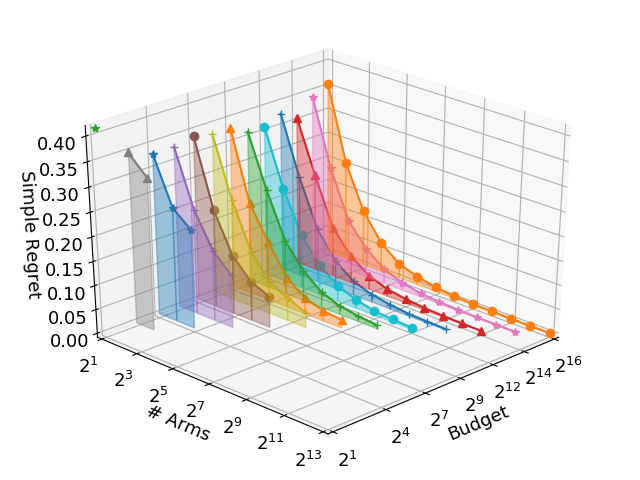
\includegraphics[width=\textwidth]{fixedbudget/figures/folder1/alpha1_beta1_unscaled.png}
	\caption{$Beta(1,1)$}
	\label{appendix:fig:sh-num-arms:alpha1_beta1_unscaled}
\end{subfigure}
\quad
\begin{subfigure}{0.4\textwidth}
	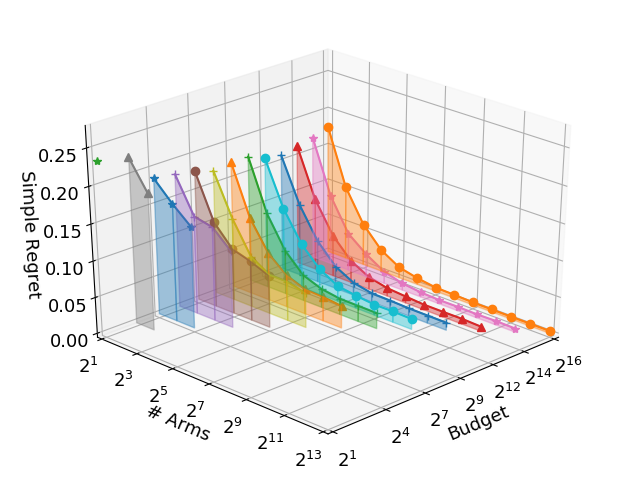
\includegraphics[width=\textwidth]{fixedbudget/figures/folder1/alpha1_beta1_scaled.png}
	\caption{$Beta(1,1)$ Scaled}
	\label{appendix:fig:sh-num-arms:alpha1_beta1_scaled}
\end{subfigure}
%
\begin{subfigure}{0.4\textwidth}
	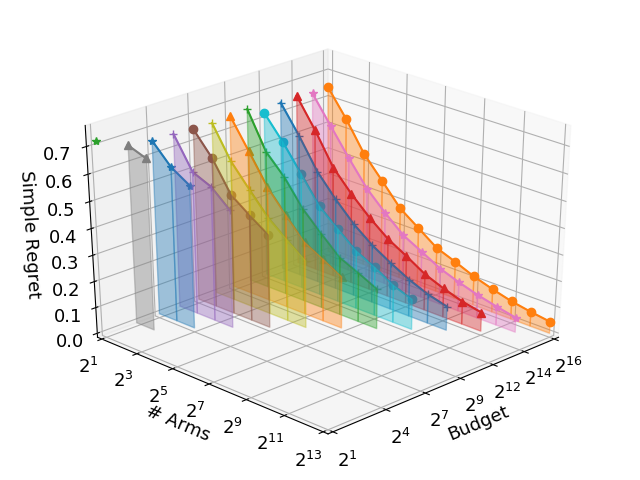
\includegraphics[width=\textwidth]{fixedbudget/figures/folder1/alpha1_beta3_unscaled.png}
	\caption{$Beta(3,1)$}
	\label{appendix:fig:sh-num-arms:alpha1_beta3_unscaled}
\end{subfigure}
\quad
\begin{subfigure}{0.4\textwidth}
	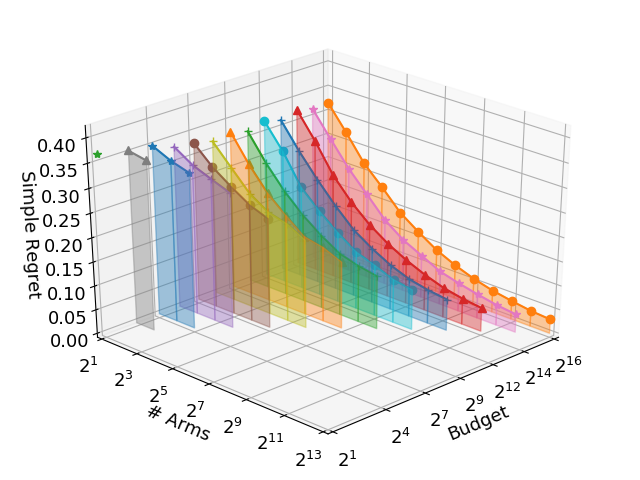
\includegraphics[width=\textwidth]{fixedbudget/figures/folder1/alpha1_beta3_scaled.png}
	\caption{$Beta(3,1)$ Scaled}
	\label{appendix:fig:sh-num-arms:alpha1_beta3_scaled}
\end{subfigure}
%
\begin{subfigure}{0.4\textwidth}
	\includegraphics[width=\textwidth]{fixedbudget/figures/folder1/{TwoSpike_0.1_0.515_0.031}.png}
	\caption{TwoSpike $\pi=10^{-1}, \epsilon=\sqrt{10^{-3}}$}
	\label{appendix:fig:sh-num-arms:TwoSpike_1}
\end{subfigure}
\quad
\begin{subfigure}{0.4\textwidth}
	\includegraphics[width=\textwidth]{fixedbudget/figures/folder1/{TwoSpike_0.01_0.55_0.1}.png}
	\caption{Two Spike $\pi=10^{-2}, \epsilon=\sqrt{10^{-2}}$}
	\label{appendix:fig:sh-num-arms:TwoSpike_2}
\end{subfigure}
%
\begin{subfigure}{0.4\textwidth}
	\includegraphics[width=\textwidth]{fixedbudget/figures/folder1/{TwoSpike_0.001_0.658_0.316}.png}
	\caption{Two Spike $\pi=10^{-3}, \epsilon=\sqrt{10^{-1}}$}
	\label{appendix:fig:sh-num-arms:TwoSpike_3}
\end{subfigure}
\quad
\begin{subfigure}{0.4\textwidth}
	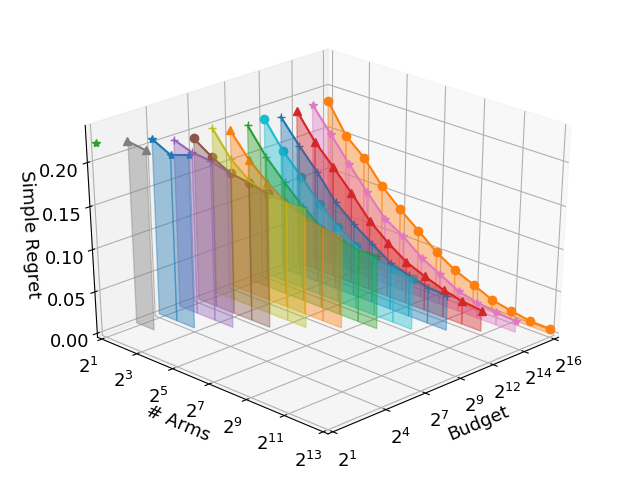
\includegraphics[width=\textwidth]{fixedbudget/figures/folder1/new_yorker.png}
	\caption{New Yorker}
	\label{appendix:fig:sh-num-arms:new_yorker}
\end{subfigure}
\label{appendix:fig:sh-num-arms}
\end{figure}

\begin{figure}
\centering
\caption{Comparison to state-of-the-art pure exploration infinite bandit algorithms}
\begin{subfigure}{0.4\textwidth}
	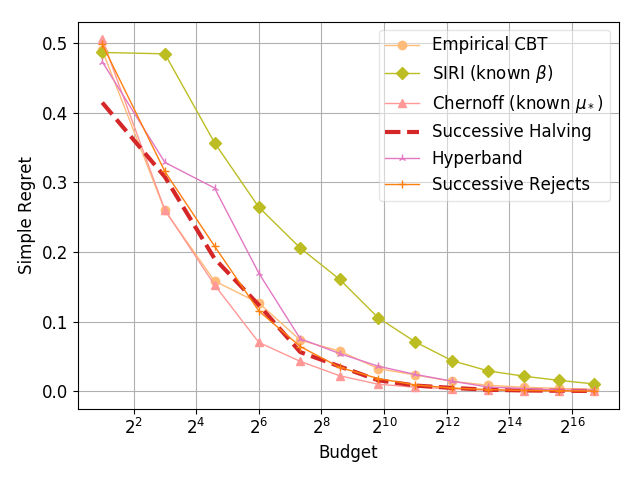
\includegraphics[width=\textwidth]{fixedbudget/figures/folder4/alpha1_beta1_unscaled.png}
	\caption{$Beta(1,1)$}
	\label{appendix:fig:sh-infinite:alpha1_beta1_unscaled}
\end{subfigure}
\quad
\begin{subfigure}{0.4\textwidth}
	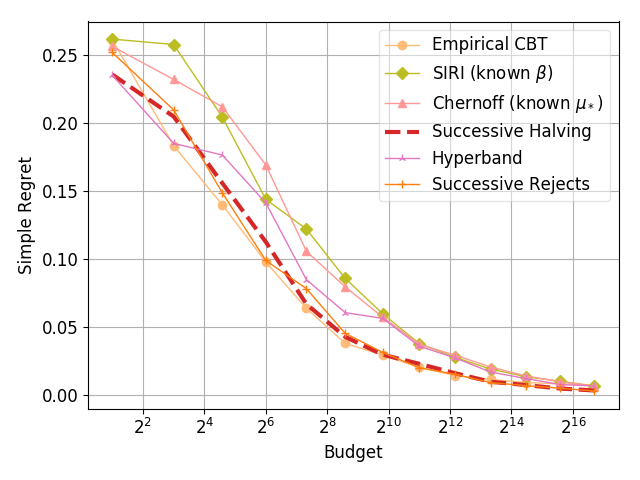
\includegraphics[width=\textwidth]{fixedbudget/figures/folder4/alpha1_beta1_scaled.png}
	\caption{$Beta(1,1)$ Scaled}
	\label{appendix:fig:sh-infinite:alpha1_beta1_scaled}
\end{subfigure}
%
\begin{subfigure}{0.4\textwidth}
	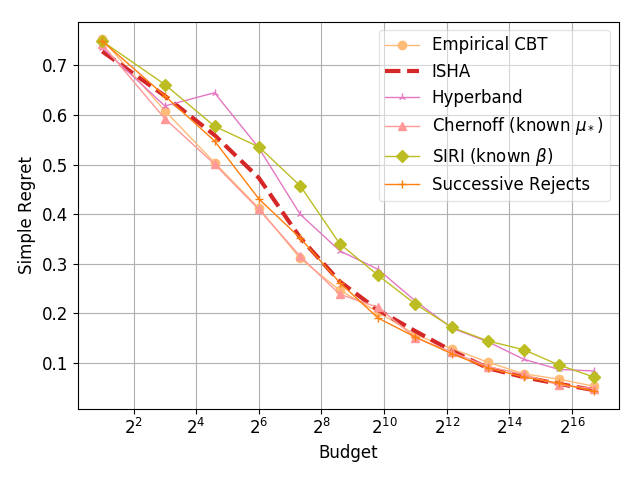
\includegraphics[width=\textwidth]{fixedbudget/figures/folder4/alpha1_beta3_unscaled.png}
	\caption{$Beta(3,1)$}
	\label{appendix:fig:sh-infinite:alpha1_beta3_unscaled}
\end{subfigure}
\quad
\begin{subfigure}{0.4\textwidth}
	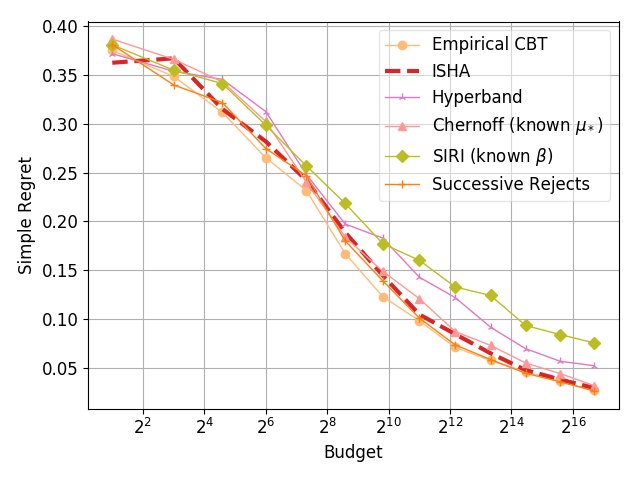
\includegraphics[width=\textwidth]{fixedbudget/figures/folder4/alpha1_beta3_scaled.png}
	\caption{$Beta(3,1)$ Scaled}
	\label{appendix:fig:sh-infinite:alpha1_beta3_scaled}
\end{subfigure}
%
\begin{subfigure}{0.4\textwidth}
	\includegraphics[width=\textwidth]{fixedbudget/figures/folder4/{TwoSpike_0.1_0.515_0.031}.png}
	\caption{TwoSpike $\pi=10^{-1}, \epsilon=\sqrt{10^{-3}}$}
	\label{appendix:fig:sh-infinite:TwoSpike_1}
\end{subfigure}
\quad
\begin{subfigure}{0.4\textwidth}
	\includegraphics[width=\textwidth]{fixedbudget/figures/folder4/{TwoSpike_0.01_0.55_0.1}.png}
	\caption{Two Spike $\pi=10^{-2}, \epsilon=\sqrt{10^{-2}}$}
	\label{appendix:fig:sh-infinite:TwoSpike_2}
\end{subfigure}
%
\begin{subfigure}{0.4\textwidth}
	\includegraphics[width=\textwidth]{fixedbudget/figures/folder4/{TwoSpike_0.001_0.658_0.316}.png}
	\caption{Two Spike $\pi=10^{-3}, \epsilon=\sqrt{10^{-1}}$}
	\label{appendix:fig:sh-infinite:TwoSpike_3}
\end{subfigure}
\quad
\begin{subfigure}{0.4\textwidth}
	\includegraphics[width=\textwidth]{fixedbudget/figures/folder4/new_yorker.png}
	\caption{New Yorker}
	\label{appendix:fig:sh-infinite:new_yorker}
\end{subfigure}
\label{appendix:fig:sh-infinite}
\end{figure}


\begin{figure}
\centering
\caption{Comparison to lil'UCB}
\begin{subfigure}{0.4\textwidth}
	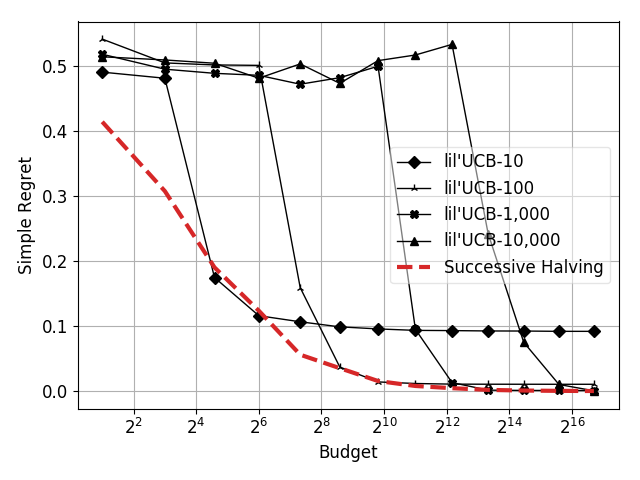
\includegraphics[width=\textwidth]{fixedbudget/figures/folder5/alpha1_beta1_unscaled.png}
	\caption{$Beta(1,1)$}
	\label{appendix:fig:sh-lilucb:alpha1_beta1_unscaled}
\end{subfigure}
\quad
\begin{subfigure}{0.4\textwidth}
	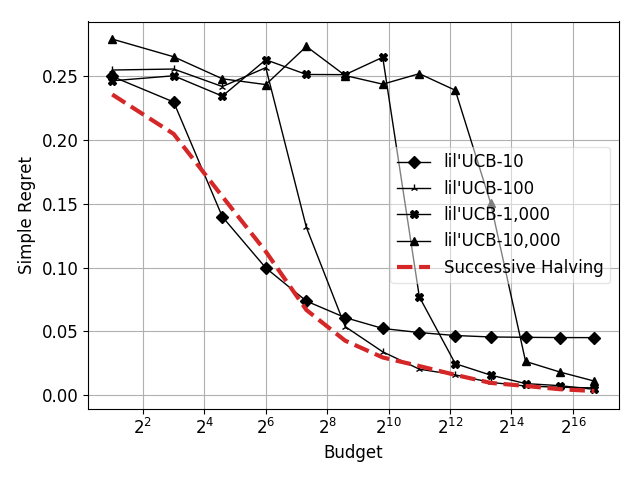
\includegraphics[width=\textwidth]{fixedbudget/figures/folder5/alpha1_beta1_scaled.png}
	\caption{$Beta(1,1)$ Scaled}
	\label{appendix:fig:sh-lilucb:alpha1_beta1_scaled}
\end{subfigure}
%
\begin{subfigure}{0.4\textwidth}
	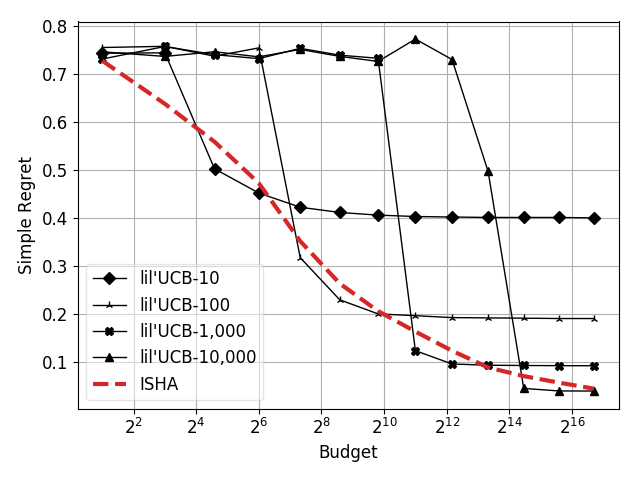
\includegraphics[width=\textwidth]{fixedbudget/figures/folder5/alpha1_beta3_unscaled.png}
	\caption{$Beta(3,1)$}
	\label{appendix:fig:sh-lilucb:alpha1_beta3_unscaled}
\end{subfigure}
\quad
\begin{subfigure}{0.4\textwidth}
	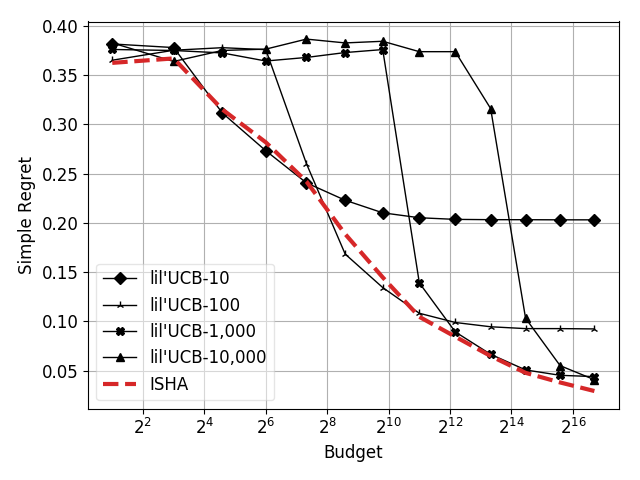
\includegraphics[width=\textwidth]{fixedbudget/figures/folder5/alpha1_beta3_scaled.png}
	\caption{$Beta(3,1)$ Scaled}
	\label{appendix:fig:sh-lilucb:alpha1_beta3_scaled}
\end{subfigure}
%
%\begin{subfigure}{0.4\textwidth}
%	\includegraphics[width=\textwidth]{figures/folder5/new_yorker.png}
%	\caption{New Yorker}
%	\label{fig:sh-lilucb:new_yorker}
%\end{subfigure}
\label{appendix:fig:sh-lilucb}
\end{figure}


\begin{figure}
\centering
\caption{Comparison to state-of-the-art explore-vs-exploit infinite bandit algorithms}
\begin{subfigure}{0.4\textwidth}
	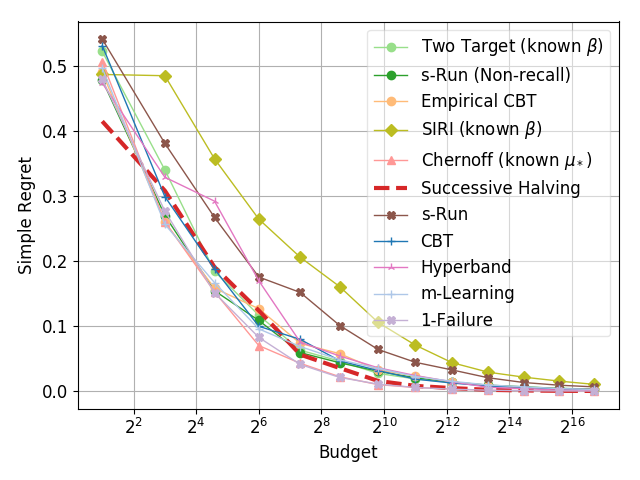
\includegraphics[width=\textwidth]{fixedbudget/figures/folder2/alpha1_beta1_unscaled.png}
	\caption{$Beta(1,1)$}
	\label{appendix:fig:sh-unscaled-alpha1_beta1_unscaled}
\end{subfigure}
\quad
\begin{subfigure}{0.4\textwidth}
	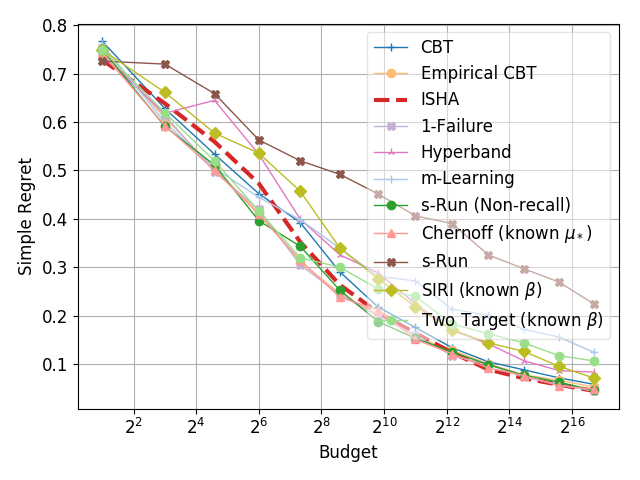
\includegraphics[width=\textwidth]{fixedbudget/figures/folder2/alpha1_beta3_unscaled.png}
	\caption{$Beta(3,1)$}
	\label{appendix:fig:sh-unscaled-alpha1_beta3_unscaled}
\end{subfigure}
\label{appendix:fig:sh-unscaled}
\end{figure}


\begin{figure}
\centering
\caption{Anytime Performance}
\begin{subfigure}{0.4\textwidth}
	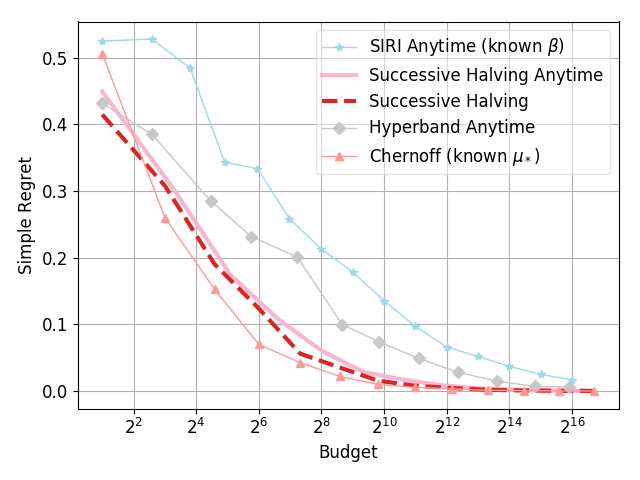
\includegraphics[width=\textwidth]{fixedbudget/figures/folder3/alpha1_beta1_unscaled.png}
	\caption{$Beta(1,1)$}
	\label{appendix:fig:sh-anytime:alpha1_beta1_unscaled}
\end{subfigure}
\quad
\begin{subfigure}{0.4\textwidth}
	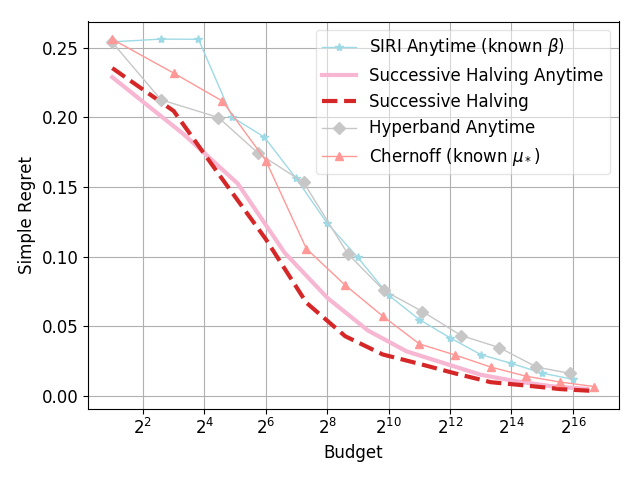
\includegraphics[width=\textwidth]{fixedbudget/figures/folder3/alpha1_beta1_scaled.png}
	\caption{$Beta(1,1)$ Scaled}
	\label{appendix:fig:sh-anytime:alpha1_beta1_scaled}
\end{subfigure}
%
\begin{subfigure}{0.4\textwidth}
	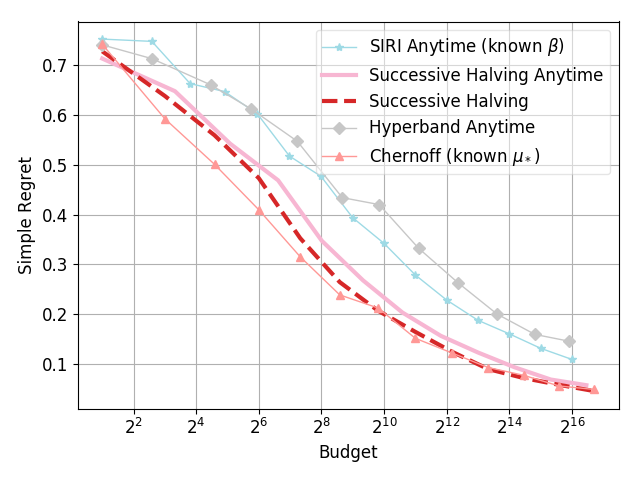
\includegraphics[width=\textwidth]{fixedbudget/figures/folder3/alpha1_beta3_unscaled.png}
	\caption{$Beta(3,1)$}
	\label{appendix:fig:sh-anytime:alpha1_beta3_unscaled}
\end{subfigure}
\quad
\begin{subfigure}{0.4\textwidth}
	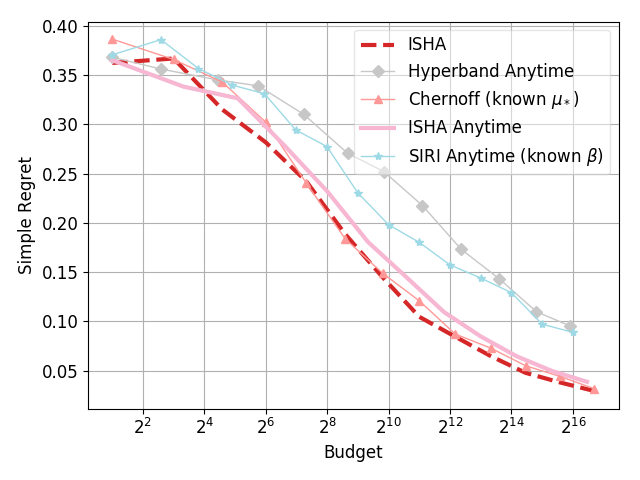
\includegraphics[width=\textwidth]{fixedbudget/figures/folder3/alpha1_beta3_scaled.png}
	\caption{$Beta(3,1)$ Scaled}
	\label{appendix:fig:sh-anytime:alpha1_beta3_scaled}
\end{subfigure}
%
\label{appendix:fig:sh-anytime}
\end{figure}

\begin{figure}
% \vspace{-2.5em}
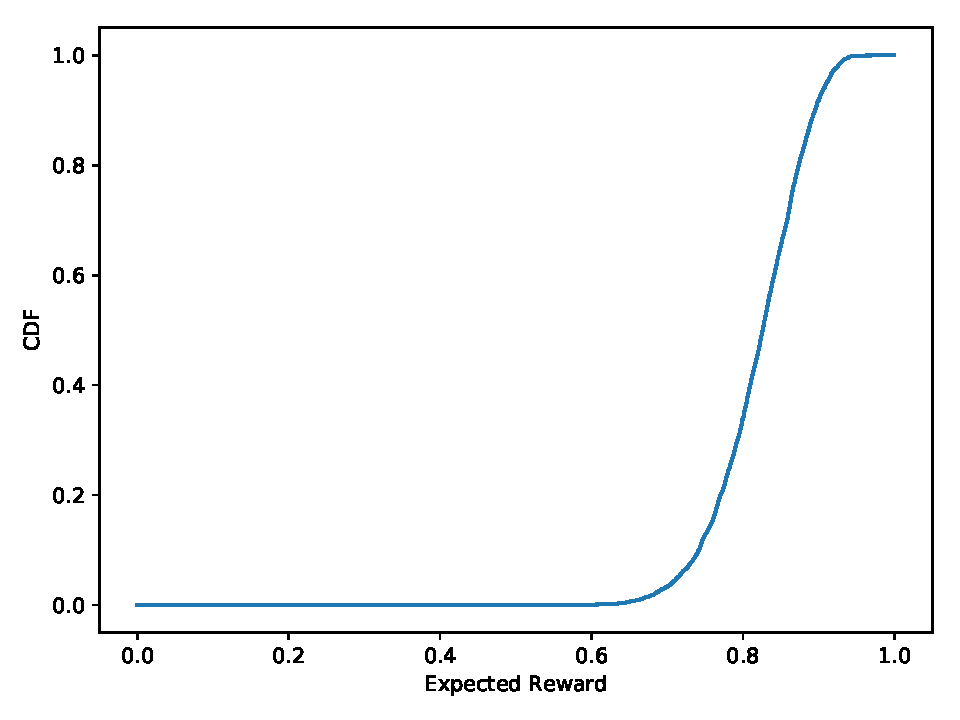
\includegraphics[width=\textwidth]{fixedbudget/figures/NY_CDF.pdf}
\caption{New Yorker CDF}
\label{fig:newyorkercdf}
\end{figure}
